\documentclass{article}
\usepackage[T1]{fontenc}
\usepackage{lmodern}
\usepackage{graphicx}
\usepackage{amsmath,amssymb}
\usepackage[a4paper,margin=2cm]{geometry}
\usepackage[absolute,overlay]{textpos}
\setlength{\TPHorizModule}{1mm}
\setlength{\TPVertModule}{1mm}
\usepackage[indonesian]{babel}
\usepackage{hyperref}
\setlength{\emergencystretch}{2em}
% unit: Halaman 44

\begin{document}

% === Halaman 44 (llm) ===

\vspace{142.56mm}

Jika $s = b$, maka mode $OFB$ $s$-bit adalah seperti pada Gambar berikut

% deskripsi: Diagram alur proses enkripsi dan dekripsi menggunakan mode Output Feedback (OFB) s-bit, yang terdiri dari dua bagian: (a) Encryption dan (b) Decryption.
% bbox normalisasi: [0.0100, 0.2800, 0.9700, 0.7600]
\begin{textblock*}{201.60mm}(2.10mm,83.16mm)
\noindent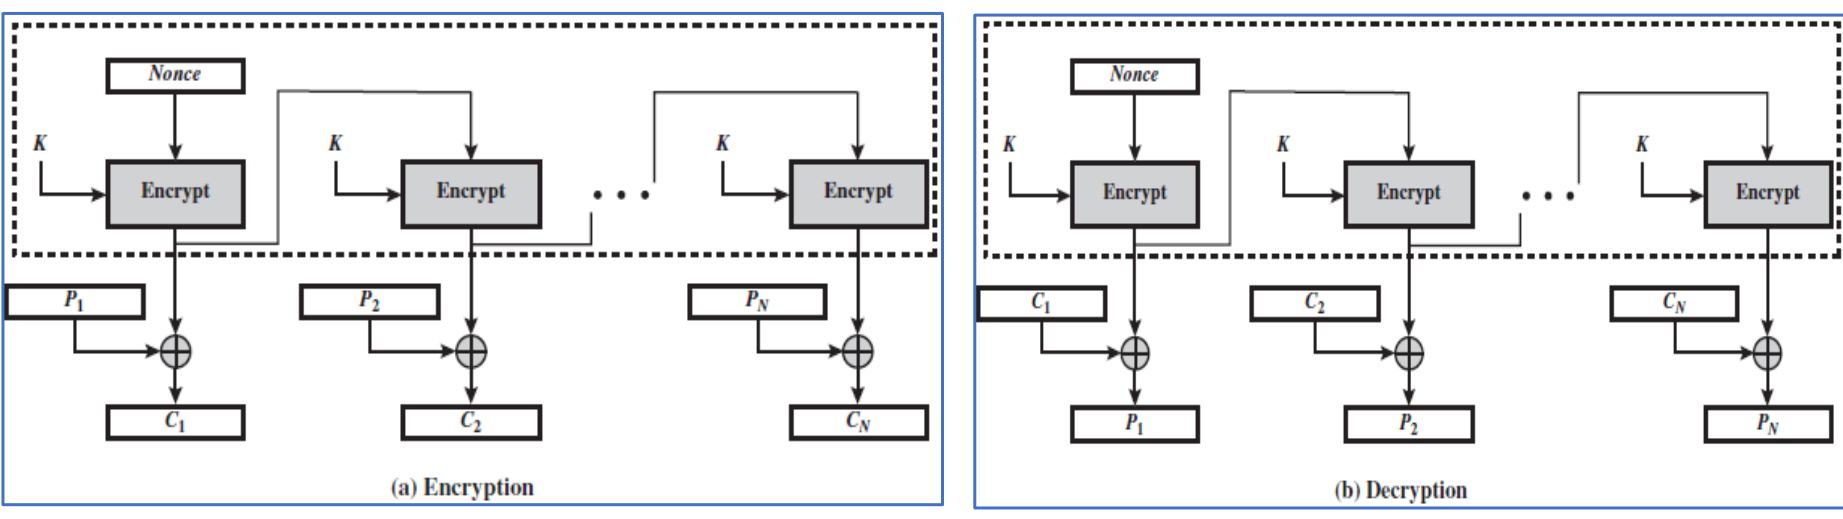
\includegraphics[width=201.60mm,height=142.56mm]{../../images/llm/page_044_img_01.png}%
\end{textblock*}

\end{document}
